
\vspace{-1.5em}
\section{相关工作}
\label{sec:related}
\vspace{-1em}

\subsubsection{2D 视频对象分割。}
视频对象分割（VOS）在视频序列中分割并跟踪目标对象，生成时间上连贯的掩码~\cite{perazzi2016benchmark, caelles2017one, voigtlaender2019feelvos, maninis2018video, wu2025denver}。早期方法依赖外观传播或光流，但在长期一致性和遮挡情况下表现受限~\cite{yang2019video, oh2019video, bhat2020learning}。近期基于记忆的架构利用时空注意力和特征检索改善对象关联~\cite{yang2021associating, cheng2022xmem, cheng2021rethinking, liu2022learning, park2022per, xu2022reliable, yang2024scalable, yang2022decoupling, li2024univs, cheng2024putting}；后续工作通过受限记忆库~\cite{zhou2024rmem}、门控线性匹配~\cite{liu2025livos}、统一 Transformer 框架~\cite{li2024onevos, zhang2025jointformer} 和动态锚点查询~\cite{zhou2024improving} 进一步提升记忆效率。新的基准~\cite{hong2023lvos} 以及全景视频~\cite{yan2024panovos}、基于点的提示~\cite{mahadevan2024point} 等特殊设置也拓宽了评估范围。

SAM2~\cite{ravi2024sam2} 是一种具有流式记忆的可提示模型，在多个基准上表现强劲。后续工作通过记忆树增强 SAM2 的长程身份保持~\cite{ding2024sam2long}，引入干扰物感知更新~\cite{videnovic2025distractor}、端侧效率~\cite{zhou2025edgetam}、文本驱动理解~\cite{cuttano2025samwise} 以及其他改进~\cite{yang2024samurai, yang2025mosam, ye2025entitysam}。并行工作还将 SAM2 与大语言模型结合，用于基于推理的分割~\cite{yuan2025sa2va, yan2024visa, bai2024one}。尽管如此，大幅视角变化、遮挡以及消失—重现事件仍会造成显著退化~\cite{ding2025mosev2, xu2018youtube, perazzi2017davis}。我们的方法通过将 3D 感知表示整合进 SAM2，解决挑战性视角和外观变化下的对象一致分割问题。

\vspace{-1em}
\subsubsection{3D 实例分割。}
主流 3D 实例分割主要有两条路线。以提议为中心的方法通过学习到的提议从点云预测实例掩码~\cite{schult2022mask3d, jiang2020pointgroup, han2020occuseg, vu2022softgroup, misra2021end, sun2023superpoint, kolodiazhnyi2024oneformer3d, takmaz2023openmask3d, piekenbrinck2025opensplat3d}，近期扩展还加入了可提示分割~\cite{zhou2024point} 和快速开放词汇识别~\cite{boudjoghra2025openyolo}。另一条互补路线通过投影逐视角掩码并跨视角合并，将 2D 结果提升到 3D~\cite{yang2023sam3d, xu2024embodiedsam, nguyen2024open3dis, boudjoghra2024open, jung2025details, xu2023neurallift, kerr2023lerf, vora2021nesf, jiang2024open, bautista2022gaudi, hsu2025openm3d, tu2023imgeonet, li2024genrc}；这些方法使用超点亲和性~\cite{yin2024sai3d}、零样本特征蒸馏~\cite{wang2024lift3d, engelmann2024opennerf}、层次化对比学习~\cite{ying2024omniseg3d, kim2024garfield} 和自我中心 Gaussian 提升~\cite{gu2024egolifter}，但在掩码整合时仍依赖带位姿的 RGB-D。

3D Gaussian Splatting 的兴起进一步促进了语义场景表示：将基础模型特征蒸馏到 Gaussians~\cite{qin2024langsplat, zhou2024feature, wu2024opengaussian, peng20243d}，为每个 Gaussian 分配身份编码~\cite{ye2024gaussian, zhai2025panogs}，最优求解 2D 到 3D 标签分配~\cite{shen2024flashsplat}，以及端到端统一提升与分割~\cite{zhu2025rethinking}。然而，纯 2D 可提示分割通常不足以处理 3D 实例，因为它没有强制跨视角一致性，导致视角不一致掩码和碎片化实例~\cite{zhao2025sam2object, xu2024embodiedsam, peng2023openscene, takmaz2023openmask3d, jia2024sceneverse}。我们的方法则直接在视频上施加 3D 感知自一致性，无需 3D 标注或点云掩码合并即可保持身份与几何。


\begin{figure*}[t]
  \centering
\vspace{-3mm}
  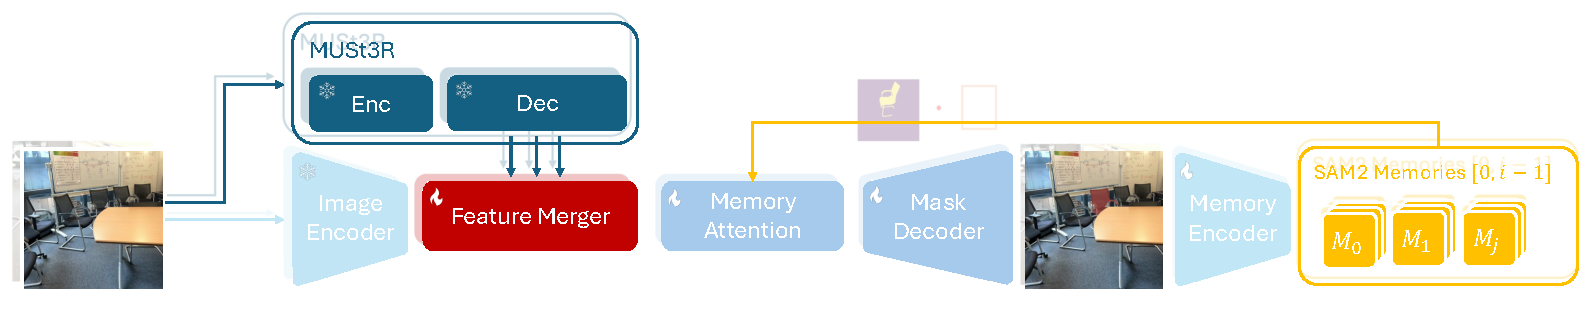
\includegraphics[width=\linewidth]{figs/pipeline.pdf}
  \vspace{-6mm}
  \caption{\textbf{3AM 流水线概览。} 
  我们的 Feature Merger 将从多视角一致性中学习、编码隐式几何对应的多层级 MUSt3R 特征，与 SAM2 的外观特征通过交叉注意力和卷积细化进行融合。融合后的几何感知表示随后经过与历史帧的记忆注意力和掩码解码，使模型在推理时无需相机位姿，也能实现空间一致的对象识别，并在大幅视角变化下保持身份。
  }
  \label{fig:pipline}
\vspace{-3mm}
\end{figure*}


\vspace{-1em}
\subsubsection{端到端 3D 感知方法。}
近期端到端 3D 重建模型可直接从 2D 输入推断几何结构~\cite{cabon2025must3r, wang2024dust3r, wang2025continuous, wang2025vggt, yang2025fast3r, chen2025long3r, leroy2024grounding, wu2025point3r, charatan2024pixelsplat, ye2024no, wang20243d, lin2025longsplat, shih2025prior, fan2025spectromotion, liu2023robust, su2024boostmvsnerfs}。DUSt3R/MASt3R 家族已被扩展到动态场景~\cite{zhang2024monst3r}、带空间记忆的增量重建~\cite{wang20253d}、前馈 Gaussian splatting~\cite{smart2024splatt3r}、高效多视角融合~\cite{tang2025mv}、实时稠密 SLAM~\cite{murai2025mast3r}、无约束运动恢复结构~\cite{duisterhof2025mast3r} 和无需训练的 4D 重建~\cite{chen2025easi3r}。前馈模型如今也覆盖了视角合成、深度估计和点云重建等任务。我们的工作并不使用这些模型输出的显式几何进行 3D 分割，而是利用它们的中间表示作为跨视角对象关联线索。

MUSt3R~\cite{cabon2025must3r} 尤其适合我们的目标，因为其在线记忆机制能够在长序列中维持多视角一致特征。我们表明，将这些特征融入 SAM2 的跟踪流程，可为 2D 可提示分割注入 3D 感知对应关系，同时保持 RGB-only 推理和在线运行能力。
